\begin{figure}[bth]
	\begin{center}
		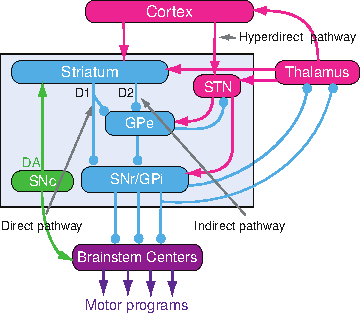
\includegraphics[width=0.7\linewidth]{ch-intro/figures/BGAnatomy}
		\caption[Anatomy of the Basal Ganglia]
		{\textbf{Schematic Anatomy of the basal ganglia.}
		The gray highlighted rectangle depicts the BG nuclei.
		Arrows show anatomical connections (\textit{red}: glutamatergic; \textit{blue}: GABAergic; \textit{green}: DAergic).
		STN:~subthalamic nucleus;
		GPe:~globus pallidus externus;
		SNc:~substantia nigra pars compacta;
		SNr:~substantia nigra pars reticulata;
		GPi:~globus pallidus internus;
		DA:~dopamine.
		Figure slightly modified from~\cite{Grillner2016BG}.
		}
		\label{fig:intro:BGAnatomy}
	\end{center}
\end{figure}